The Human Brain Project, a European Flagship, is developing a European research infrastructure advancing brain research, medicine, and brain-inspired information technology for both industry and science.
The project is now entering its third phase, with over 100 partnering institutions from over 20 countries in Europe, as well as over 100 partering projects.
There are 12 subprojects in HBP, that span the development of six ICT-based Platforms.
One of these six platforms is the Neuromorphic Computing (NMC) Platform, with two systems;
the mixed-signal VLSI BrainScaleS (Brain-inspired multiScale computation in neuromorphic hybrid systemS) and the massively parallel digital SpiNNaker (Spiking Neural Network architecture).\cite{amunts_human_2016}.
As mentioned in \vref{sect:eh} the BrainScaleS system is based on physical, analog, models of neurons and synapses, while the programmable interconnections are digital \cite{zoschke_full_2017}
The system is has an accelerated speed-up factor of 1000-10000 compared to biology, as relevant time constants are scaled down, with the goal of emulating various evolutionary mechanisms of the brain in one single set-up.
The emphasis on the system is to use our knowledge of biology to model physical electronic neurons that neuroscientists can access and study at a much higher rate, due to our limited access to biological neurons.
In addition to brain research, it is thought that this neuromorphic system will enable new applications in robotics, artificial intelligence and human-machine interfaces.
Using a physical model keeps a one-to-one relationship between the neurons and synapses of the biological example and the model,
preserving the fault tolerance concerning loss which is inherent in the biological brain.
By using only a few transistors to emulate the neuron's differential equations compared to several millions involved in the same task while solving these equations numerically in a microprocessor core, the power consumption is reduced by several orders of magnitude.
\cite{schemmel_wafer-scale_2010}
As the neurons on the HICANN chip is emulated with analog electronics rather than with a high number of arithmetic operations, the circuitry is power efficient, and a complete HICANN consumes only $1.3 W/cm^2$.
The wafer module as a whole is designed for a worst-case power consumption of 2 kW.
\cite{zoschke_full_2017}

The accelerated network has extreme requirements in terms of communication bandwith, and this is met by employing wafer scale integration for the inter-chip connectivity\cite{zoschke_full_2017}.
The wafer scale integration is in accordance with the proposal of C. Mead, which proposed interconnecting chips with analog components by integrating the production wafer \cite{mead_neuromorphic_1990}.
The base chips on the BrainScaleS wafer is the HICANN, see \vref{sect:hicann}.
A single 200 mm wafer carries 384 HICANN chips, and is mounted into a module which delivers power and handles data traffic using FPGAs.
In addition to delivering signals to and from each wafer, the FPGAs are used to configure the chips. \cite{zoschke_full_2017}.
On one wafer module there is 48 FPGA module, each equipped with Gigabit-Ethernet, to handle the high amount of event data per time that will occur on the accelerated system.
12 Gigabit connections are routed to each edge of the module, respectively, to communicate with other wafer modules and the host computer.
On the wafer, one FPGA controls 8 HICANN chips that together account for one reticle.
Every HICANN has two full-duplex serial LVDS links with separate clock and data lines to the FPGA module, and each link is capable of transmitting two GBit/s.
The input count per neuron can be increased to 14336 synapses per neuron, by combining up to 64 adjacent neurons.
This leads to a transmission requirement of 1.4 GEvents/s per neuron, which is why the silicon wafer is kept as a whole, to produce shorter transmission lines and a lower capacitive load.
The current BrainScaleS implementation,c at the Kirchhoff-Institute for Physics at Heidelberg University, enables up to 20 wafer modules, with up to 200 000 neurons and 40 000 000 synapses, per wafer.
\cite{zoschke_full_2017}

\subsection{The Neuron Model}\label{sect:adexp} at the basis of the HICANN is called the Adaptive Exponential Integrate-and-Fire model (AdExp) \cite{brette_adaptive_2005}.
The AdExp model was co-developed by the FACETS project \cite{schemmel_wafer-scale_2010}, a pre-decessor to the BranScaleS project, which is now part of the NMC platform of HBP.
The model contains several additions compared to the standard Integrate-and-Fire model (IAF):
\begin{equation}\label{eq:adexp-membrane}
-C_m\frac{dV}{dt} = g_l(V-E_l) - g_l\Delta_{th}exp(\frac{V-V_{th}}{\Delta_{th}}) + g_e(t)(V-E_e)+g_l(t)(V-E_i)+w(t)
\end{equation}
The variables $C_m, g_l E_l, E_e$ and $E_i$ are the membrane capacity, the leakage conducatance and the leakage, exciatory and inhibitory reversal potentials.
The variables $g_e(t)$ and $g_i(t)$ represent the total excitatory and inhibitory synaptic conductances.
The addition to the standard IAF model is introduced as the \textit{exponential} term on the right hand side of the equation, which models the near-asymptotic growth of the membrane potential under certain conditions.
The \textit{treshold potential} $V_{th}$ represents the critical value above which this rapid growth can occur, and the \textit{slope factor} $\Delta_{th}$ determines the rapidness of the triggered growth.
Such a situation is interpreted as a spike, and each time a spike is detected, a separately generated output event signal is transmitted to possible connected target neurons or recording devices, and the membrane potential is forced to a reset potential $V_{reset}$ by an adjustable reset conductance.
A second equation describes the temporal evolution of the socalled \textit{adaption current} $w(t)$:
\begin{equation}\label{eq:adexp-adaption}
-\tau_{w}\frac{dw}{dt} = w(t) - a(V-E_l)
\end{equation}
Every time a spike is emitted by the neuron, $w$ changes its value: $w \rightarrow w + b$.
The time constant and the efficacy of the so-called \textit{sub-treshold} adaption mechanism are given by $\tau_w$ and $a$, while $b$ defines the amount of so-called \textit{spike-triggered} adaption.
The exponential term of equation \ref{eq:adexp-membrane} and the adaption function of equation \ref{eq:adexp-adaption} can be deactivated to reduce the AdExp model to the standard IAF model.
\cite{schemmel_wafer-scale_2010}\cite{brette_adaptive_2005}

\cref{fig:adexp-circuit} shows the individual circuit components and \cref{fig:adexp-firing} illustrates the firing modes of this neuron circuit.
In the currently operative implementation of BrainScaleS, BSS-1, the neurons are implemented in a 180 mm CMOS technology.
The system is designed to be scalable with newer generations of CMOS technology and HICANN chips \cite{zoschke_full_2017}.
The hardware implementation of the neuron is described in detail in \cite{millner_vlsi_2010},
which also reports that the emulation of an IAF neuron with the implemented hardware is 3000 times more power efficient, and accelerated by a factor of 10 000, when compared to a Izhikevich neuron simulated on a supercomputer \cite{millner_vlsi_2010}.
The Izhikevich neuron is a very popular model because it gives accurate representation of a neurons functionality while being simple to model \cite{schuman_survey_2017}.

\begin{figure}  \centering
  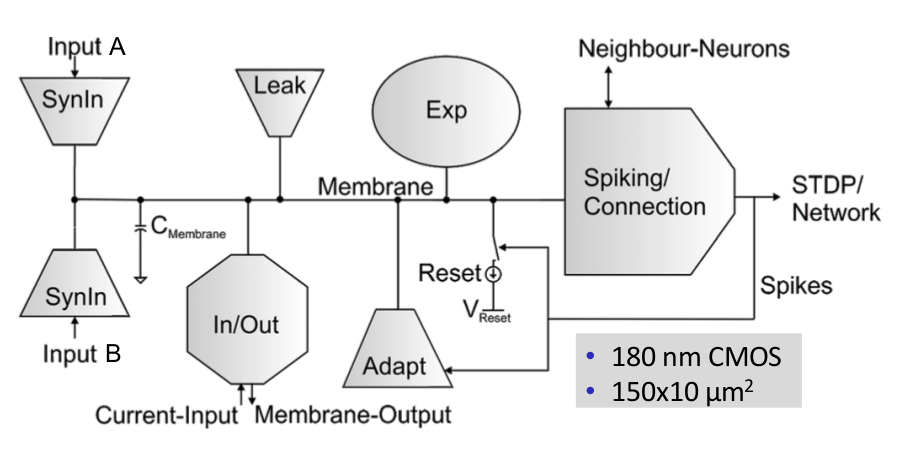
\includegraphics[width=.8\textwidth]{adexp-circuit}
    \label[figure]{fig:adexp-circuit}
    \captionof{figure}{Schematic diagram of the AdExp neuron circuit, taken from \cite{schemmel_wafer-scale_2010}.}
\end{figure}%
\begin{figure}  \centering
  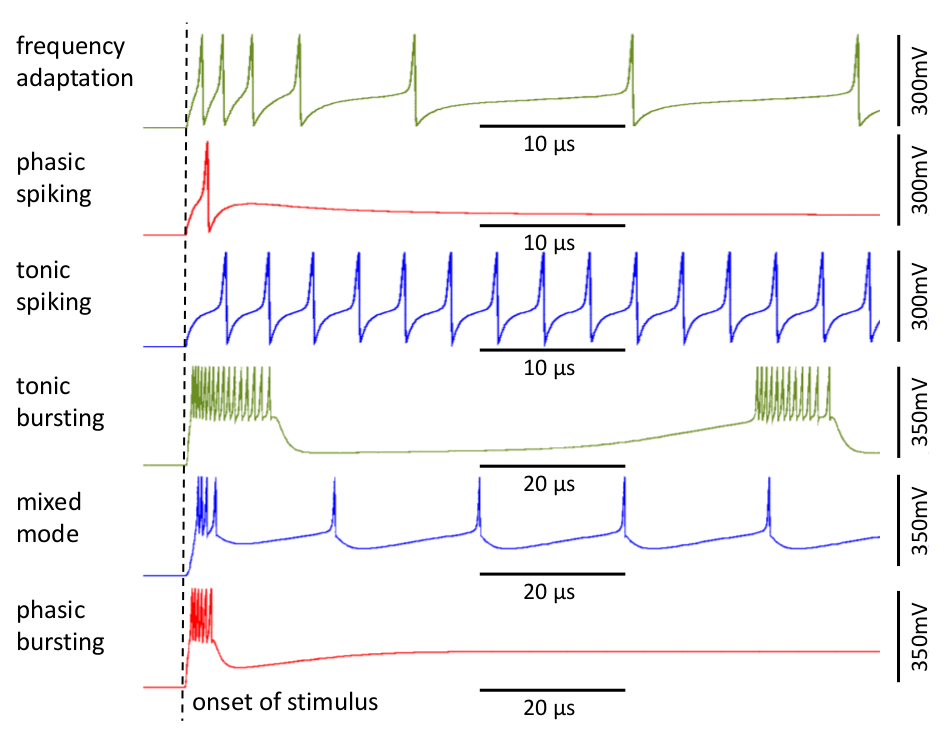
\includegraphics[width=.9\textwidth]{adexp-firing}
    \label[figure]{fig:adexp-firing}
    \captionof{figure}{Example of firing modes of the AdExp neuron circuit, taken from \cite{schemmel_wafer-scale_2010}.}
\end{figure}

\subsection{Communication} on a wafer happens on several levels; There is the communication happening between the local neurons and synapses, then there is Layer 1 (L1) and Layer 2 (L2) channels depending on how far the communication reaches.
The nature of inter-neuron communication is discussed here as it is of interest when considering how close the system is to nature,
but also to any analyzis involving Integrated Information Theory, \vref{sect:iit}.

The neuron circuits are integrated together with their respective synapses in a structure called the Analog Network Core (ANC), shown in \cref{fig:anc}.
The neurons are constructed by Dendrite Membrane (DenMem) circtuis that allow neurons with up to 14336 synaptic inputs per neuron.
The synaptic weights, stored in a four bit SRAM, are represented by a current generated by a DAC.
Short-Term Depression (STD) and Spike-Timing Dependent Plasticity (STDP) are implemented by the use of capacitors modulating the signals, and by an algorithm that manipulates the digitally stored weights.
A schematic diagram of the synaptic circuit can be seen in \cref{fig:synapse}, where $g_max$ is a programmable analog parameter controlling the scale of the DAC.
In each ANC, the communication is asynchronous and mixed-signal.
The cores are highly integrated systems working in a contiuous-time mode.
\cite{schemmel_wafer-scale_2010}

\begin{figure}  \centering
  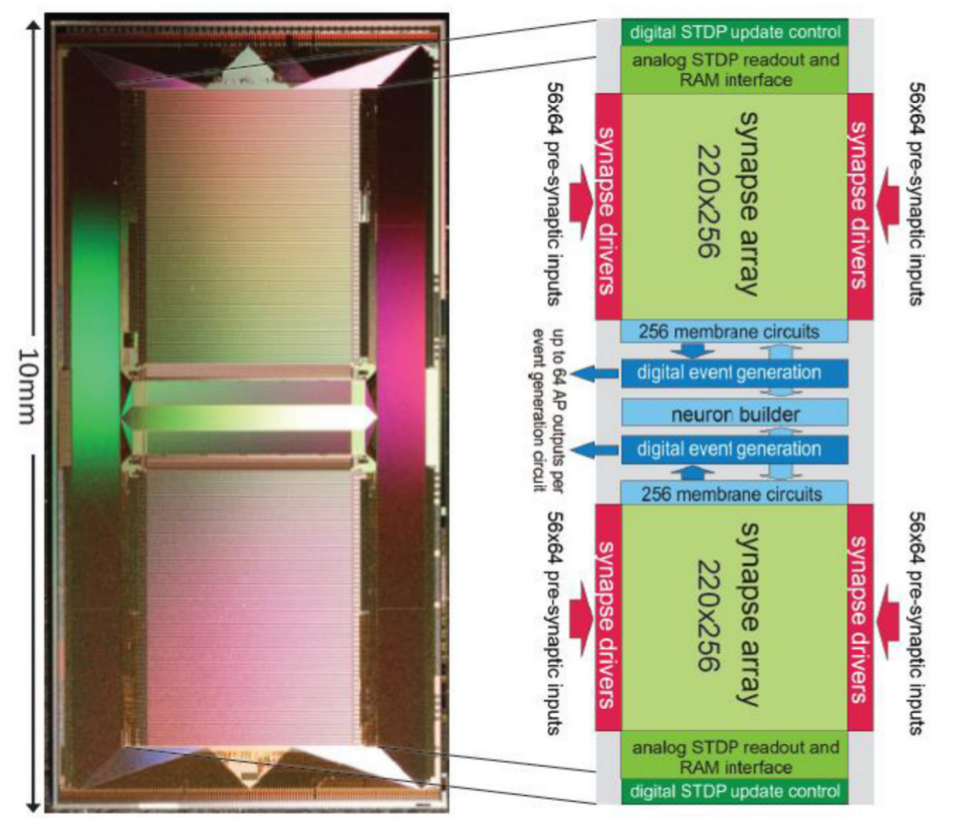
\includegraphics[width=.8\textwidth]{anc-diagram}
  \label[figure]{fig:anc}
  \captionof{figure}{To the left is a single HICANN chip, and to the right is diagram of the ANC which is located at the center of the chip, taken from \cite{thakur_large-scale_2018}.}
\end{figure}
\begin{figure}  \centering
  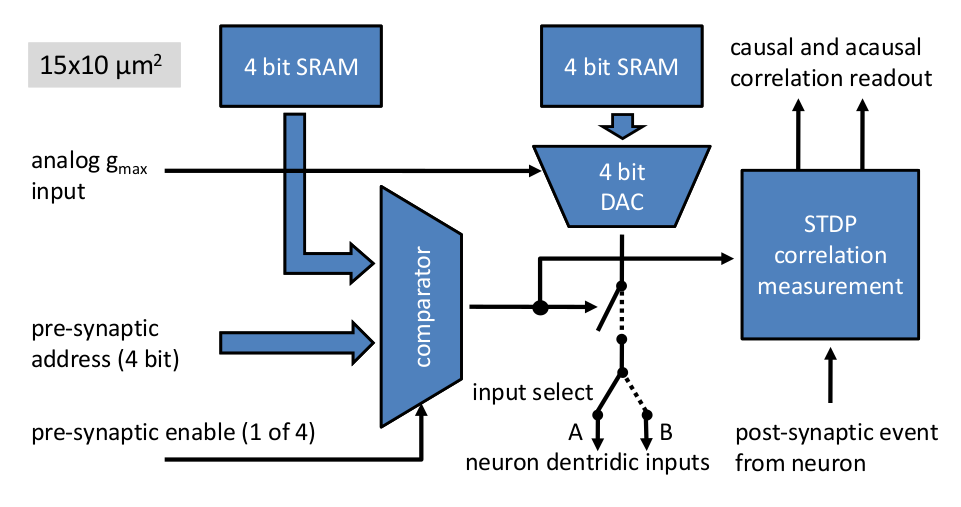
\includegraphics[width=.8\textwidth]{synapse-circuit}
  \label[figure]{fig:synapse}
  \captionof{figure}{Schematic diagram of a synapse circuit, taken from \cite{schemmel_wafer-scale_2010}.}
\end{figure}

Between ANCs there is the L1 channel, a real-time, serial event protocol operating at up to 2 Gb/s.
The protocol uses two time-frame bits and 6 address data bits, and is designed for continuous-time transmission \cite{schemmel_wafer-scale_2008}.
This digital protocol was implemented to limit the power consumption \cite{schemmel_wafer-scale_2010}.
To support the channel density requirements of an accelerated system where each neuron can receive over 10k pre-synaptic inputs, Wafer-Scale integration was selected \cite{schemmel_wafer-scale_2010}.
The solution of the Wafer-Scale integration is explained in detail in \cite{zoschke_full_2017} and \cite{thakur_large-scale_2018}.
The inter-ANC communication on a wafer is real-time, serial and only dependent on the states of the local circuits involved.

To allow for inter-wafer communication, each HICANN chip has a L2 channel.
Due to latency issues involved with real-time long-range communication, L2 is based on packets-switching and digitzed time stamps \cite{schemmel_wafer-scale_2010} \cite{thakur_large-scale_2018}.
This digital communication in-between wafers, or with the host computer, is handled by FPGAs \cite{zoschke_full_2017}.
Therefore, inter-neuron communication between wafers has a lower level of integration.










\subsection{Communication} between neurons
